\chapter{Математические модели}
Решение рассматриваемой задачи, основанное на степенной связи интенсивности напряжений и скоростей деформации ползучести при напряжениях, не превосходящих предела текучести материала, представлено в монографии Л.М.~Качанова [\ref{kachanov}].
Решение задачи о деформировании мембраны в стесненных условиях при учете упрочнения материала приведены в монографиях Н.Н.~Малинина,[\ref{malinin}] и К.И.~Романова [\ref{romanov}]. Известные работы [\ref{malinin},\ref{jerebcov}] допускают появление нефизичных бесконечных напряжений ($\sigma_u \to \infty$) в начальный момент времени, для их исключения в данной работе дополнительно учитывается мгновенное деформирование.
В [\ref{teraud_dis}, \ref{teraud}] приведено решение рассматриваемой задачи при различных граничных условиях, однако только для клиновидной матрицы. В данной работе приводится обобщение результатов, полученных в [\ref{teraud_dis}, \ref{teraud}], на случай криволинейной матрицы. Напряженное состояние мембраны можно считать безмоментным. Поскольку длина мембраны значительно превосходит её ширину, можно считать, что реализуется случай плоской деформации.

\section{Деформирование внутри криволинейной матрицы \label{section_1_1}}

	\subsection{Первая стадия}

Первая стадия~--- стадия мгновенного упругого деформирования позволяет моделировать процесс деформации в начальный момент времени, для исключения бесконечных
	напряжений при $t \sim 0$.
	Упругое деформирование мембраны описывается c помощью закона Гука при сложном напряженном состоянии при учете несжимаемости материала мембраны.
	
	
	Вводим безразмерные переменные:
	\begin{equation}
		\overline{q} = \dfrac{q}{\sigma_b}, \;
		\overline{H} = \dfrac{H}{H_0}, \;
		\overline{H}_0 = \dfrac{H_0}{a}, \;
		\overline{t} = \dfrac{\sqrt 3}{2}Ct,\;
		k = \dfrac{E}{\sigma_b},\;
		\overline{\rho} = \dfrac{\rho}{H_0},
	\end{equation}
	где $H$ ~--- толщина мембраны в произвольный момент времени, $H_0$~--- толщина мембраны при $t = -0$, $q$~--- давление, $2a$~--- ширина,
	$E$~--- модуль Юнга,  $H$ и  $\rho$~--- толщина и радиус кривизны мембраны.
	При дальнейшем анализе черточки над безразмерными величинами в этом пункте  опустим. Так как вывод формул описан в работах  [\ref{teraud_dis}, \ref{teraud}]
	и совпадает с нашим решением, приведем только итоговый результат, описывающий связь давления $q$ и мгновенно появляющегося угла $\alpha_1$,
	также приведены характеристики, описывающие состояние мембраны($H_1$~--- толщины и $\sigma_{\theta1}$):

	\begin{equation}
	\begin{split}
		q = \dfrac43 H_0k\sin(\alpha_1)\left(1-\dfrac{\sin(\alpha_1)}{\alpha_1} \right), \\
		H_1 = \dfrac{\sin(\alpha_1)}{\alpha_1},\\
		\sigma_{\theta1} = \dfrac{q}{H_1H_0\sin(\alpha_1)},
	\end{split}
	\label{guk_deformation}
	\end{equation}
	
	Следует отметить, что соотношения (\ref{guk_deformation}) позволяют исключить бесконечные напряжения в начальный момент времени.
	Так же следует отметить, что в работе расчеты этих значений для материала были произведены с помощью программного средства Maxima.
	 
	\subsection{Вторая стадия}

	\begin{figure}[h!]
		\begin{minipage}[h]{0.48\linewidth}

				
				\def\svgwidth{\columnwidth}
				\center{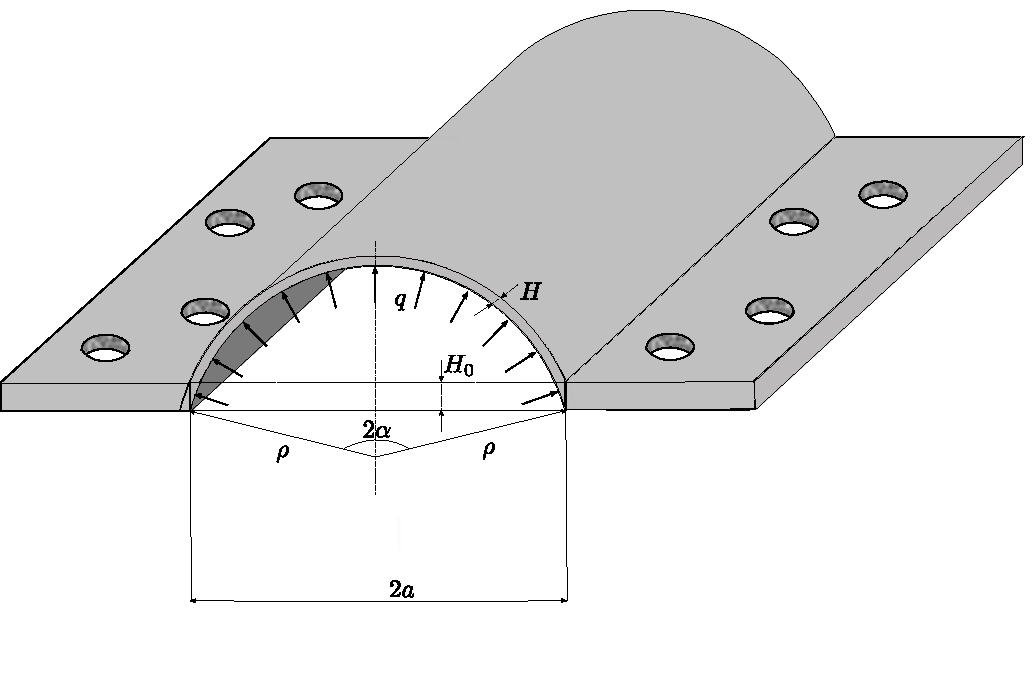
\includegraphics[width=1.0\linewidth]{images/free_membrane.pdf}}

			\caption{ Свободное деформирование } 
		\end{minipage}
		\hfill
		\begin{minipage}[h]{0.48\linewidth}	
		Вторая стадия~--- стадия свободного деформирования позволяет моделировать 
    	деформацию мембраны вплоть до её касания стенок матрицы, что соответствует углу раствора $2\alpha_2$. Подробное описание вывода 
    	соотношений описано в работах  [\ref{teraud_dis}, \ref{teraud}], поэтому приведем то соотношение, которое было рассмотрено и реализовано 
    	в работе:
		\begin{equation}
        	t = \int\limits_{\alpha_1}^{\alpha}\left(\dfrac 1\alpha - \ctg\alpha \right)\left( \dfrac{2H_0\sin^2\alpha}{\sqrt 3 q\alpha} 
        	\right)^n\,d\alpha
	        \label{free_deformation_formula}
	    \end{equation}
	
		\end{minipage}
		\label{free_deformation_pic}
	\end{figure}
	
	
	Для анимированного моделирования деформации мембраны требовались промежуточные
	расчеты по формуле (\ref{free_deformation_formula}), которые были произведены методами, описанными в пунктах: \ref{gauss}, \ref{simpson}
	\newpage
	\subsection{Третья стадия}
	\begin{figure}[h!]
		\begin{minipage}[h]{0.48\linewidth}

				
				\def\svgwidth{\columnwidth}
				\center{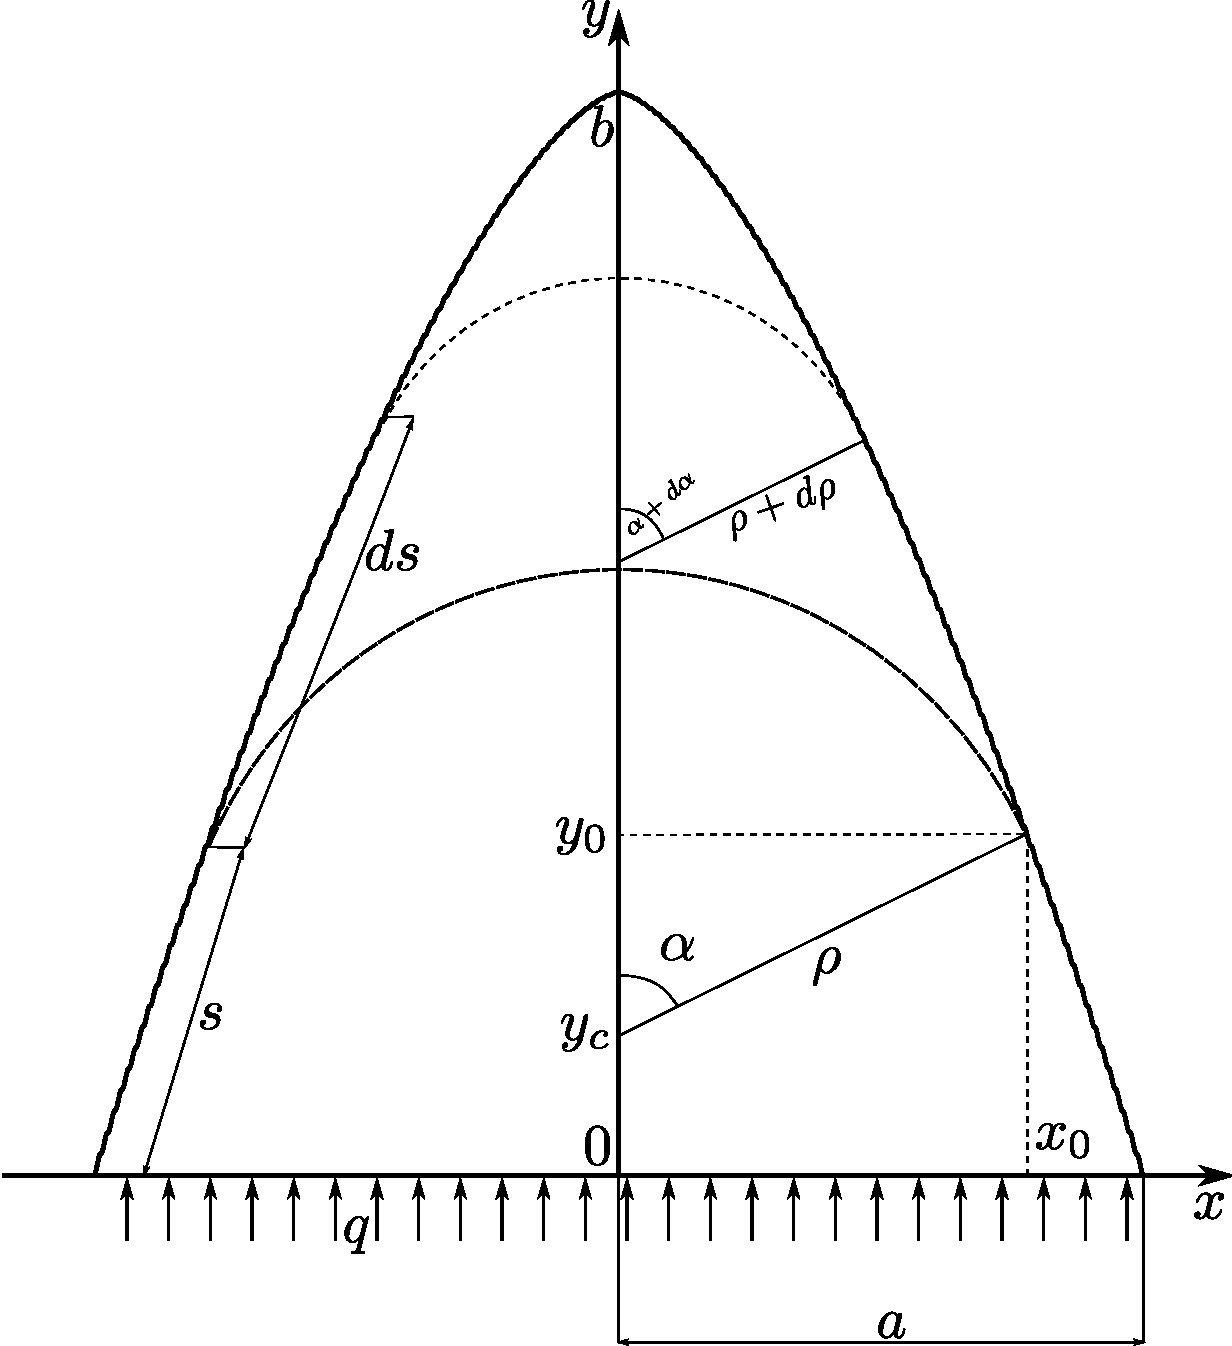
\includegraphics[width=1.0\linewidth]{images/quad_matrix.pdf}}
				\label{quad_matrix_pic}
			\caption{ Стесненное деформирование } 
		\end{minipage}
		\hfill
		\begin{minipage}[h]{0.48\linewidth}	
Началом стесненного деформирования (третья стадия) считается момент времени, при котором мембрана впервые касается матрицы. При исследовании этой стадии рассматривается идеальное скольжение и прилипание мембраны относительно стенок матрицы,  поверхность которой задана уравнением $\overline{y} = f(\overline{x}) = \overline{b}(1-(\overline{x})^k)$, $x$ и $y$ характерные размеры матрицы (\ref{quad_matrix_pic}), $\overline{x} = \frac x a$, $\overline{y} = \frac y a$,$b$~--- глубина матрицы (рис. 1) $\overline{b} = \frac b a$. При этом на матрицу будет наложено ограничение, аналогичное 
[\ref{jerebcov}]: кривизна кривой должна монотонно увеличиваться от точки $a$ до $0$, для того, чтобы зона стесненного деформирования оставалась одиночной и непрерывной.
	
		\end{minipage}
		\label{quad_matrix_pic}
	\end{figure}
	
	
Рассмотрим аналогично [\ref{jerebcov}] два близких деформированных состояния:
одно  с радиусом $\rho$ и длиной участка контакта $s$ и второе $\rho+d\rho$ и длиной участка контакта $s+ds$. Основываясь на геометрических соображениях (рис. \ref{quad_matrix_pic}), получим соотношения, характеризующие два близких состояния в данных координатных осях:
\begin{eqnarray}
\left. 
\begin{split}
\rho(x_0) &= \sqrt{(y_0-y_c)^2 + x_0^2};\; d\rho = \rho'_{x_0}dx_0\\
s(x_0) &= \int\limits^1_{x_0}\sqrt{1+f_x'^2}\,dx; \; ds = s'_{x_0}dx_0\\
\alpha(x_0)&= \dfrac{\pi}{2} - \arctg(g'_{x_0});\; d\alpha = \alpha'_{x_0}dx_0
\end{split}
\right\}
\end{eqnarray}

где $H$ ~--- толщина мембраны, $q$~--- давление, $H_0$~--- начальная толщина, $C$~---  константа материала, $a$~--- ширина, $x_0$~--- крайняя точка касания мембраны стенок матрицы, $\rho=\rho(x_0), \alpha=\alpha(x_0)$~--- радиус кривизны и угол раствора свободной части мембраны, $s=s(x_0)$~--- длина участка контакта,
$g(x_0)$~-- нормаль к функции профиля матрицы. 
Учитывая идеальное скольжение мембраны вдоль стенок матрицы, её геометрических характеристиках, получим соотношение для окружной деформации ползучести:

\begin{equation}
p_\theta = \dfrac{\rho d\alpha +\alpha d\rho+ds}{\rho\alpha+s}
\label{deformation_quad_matrix}
\end{equation}
Каждое из слагаемых числителя (\ref{deformation_quad_matrix}) содержит $dx_0$, следовательно можно сгруппировать и ввести обозначения: 
\begin{equation}
\rho d\alpha + \alpha d\rho +ds = B_1(x_0)dx_0;\; \rho\alpha+s = B_2(x_0).
\end{equation}

Тогда 
\begin{equation}
	dp_\theta = \dfrac{B_1(x_0)dx_0}{B_2(x_0)}
	\label{deformation_quad_matrix_ideal}
\end{equation}
 
 С помощью (\ref{deformation_quad_matrix_ideal}) вычисляем характеристики деформированного состояния:
 \begin{equation}
 \dot{p_\theta} = \dfrac{B_1}{B_2}\dfrac{dx_0}{dt};\;
 \dot{p_u}  = \dfrac{2}{\sqrt3} \dfrac{B_1}{B_2}\dfrac{dx_0}{dt}
 \end{equation}
 
 Аналогично выводам [\ref{jerebcov}], из условия несжимаемости плоского деформированного состояния получаем:
 \begin{equation}
 H=H_1\exp\left(\int\limits_1^{x_0}\dfrac{B_1}{B_2}dx_0\right)
  \label{quad_matrix_h}
 \end{equation}
 
 Интенсивность напряжений будет:
 \begin{equation}
 \sigma_u = \dfrac{\sqrt 3}{2}\sigma_\theta = \dfrac{\sqrt 3}{2}\dfrac{q\rho}{H}
 \label{sigma}
 \end{equation}
 
 Подставляя (\ref{deformation_quad_matrix_ideal}), (\ref{sigma}) в (\ref{main_equation}) получим выражение, характеризующее зависимость $x_0(t)$:
 
 \begin{equation}
   t = t_1 + \int\limits^{x_0}_1 \left[ \dfrac{2H}{\sqrt3 q \rho} -1\right]^n\dfrac{B_1}{B_2}\,dx_0,
   \end{equation}
где $t_1$~-- время окончания стадии свободного деформирования.   
Выражение подлежит численному исследованию, результаты которого приведены \ref{chapter_2}.

В случае постепенного прилипания контактная часть мембраны(с переменной толщиной)
является жесткой, недеформированной, а свободная часть мембраны(с постоянной толщиной), представляет собой часть дуги окружности.
Окружная деформация примет вид:
\begin{equation}
p_\theta = \dfrac{\rho d\alpha +\alpha d\rho+ds}{\rho\alpha}
\label{stick_deformation_quad_matrix}
\end{equation}

Проведя обозначения, аналогичные случаю скольжения получим: 
\begin{equation}
\rho d\alpha + \alpha d\rho +ds = B_1(x_0)dx_0;\; \rho\alpha = B_3(x_0).
\end{equation}

Тогда 
\begin{equation}
	dp_\theta = \dfrac{B_1(x_0)dx_0}{B_3(x_0)}
\label{stick_deformation_quad_matrix_final}
\end{equation}

Основные характеристики процесса формирования определяются аналогично случаю скольжения, при замене (\ref{deformation_quad_matrix_ideal}) 
на (\ref{stick_deformation_quad_matrix_final}). Обозначим только основную зависимость точки крайней точки касания матрицы от времени:

 \begin{equation}
   t = t_1 + \int\limits^{x_0}_1 \left[ \dfrac{2H}{\sqrt3 q \rho} -1\right]^n\dfrac{B_1}{B_3}\,dx_0,
   \end{equation}
\section{Деформирование внутри матрицы с вертикальными стенками и плоским днищем}
	\subsection{Первая и вторая стадия}
		Первая и вторая стадия не имеют отличительных особенностей по сравнению 
		с моделированием деформирования внутри криволинейной матрицы. Поэтому 
		при вычислениях были взяты формулы (\ref{guk_deformation}) и (\ref{free_deformation_formula}).
	\subsection{Третья и четвертая стадия}
	
		\begin{figure}[h!]
		\begin{minipage}[h]{0.48\linewidth}
			
				\def\svgwidth{\columnwidth}
				\center{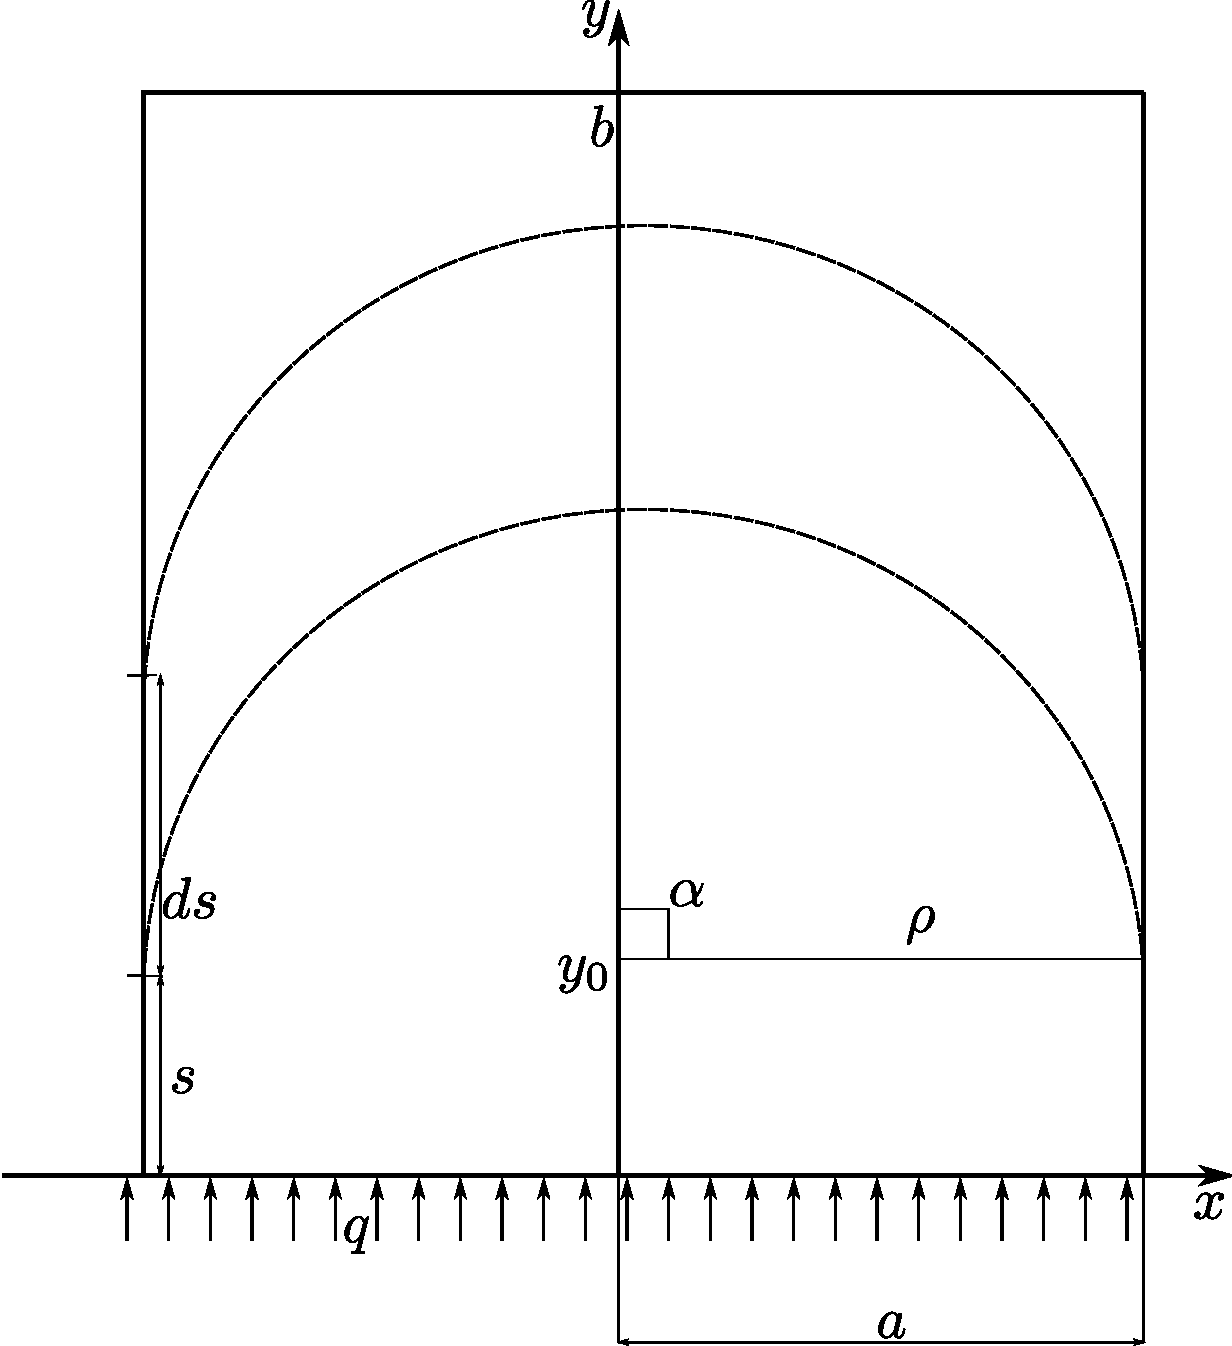
\includegraphics[width=1.0\linewidth]{images/vert_matrix.pdf}}
				\caption{ Третья стадия } 
		\end{minipage}
		\hfill
		\begin{minipage}[h]{0.48\linewidth}	

				\def\svgwidth{\columnwidth}
				\center{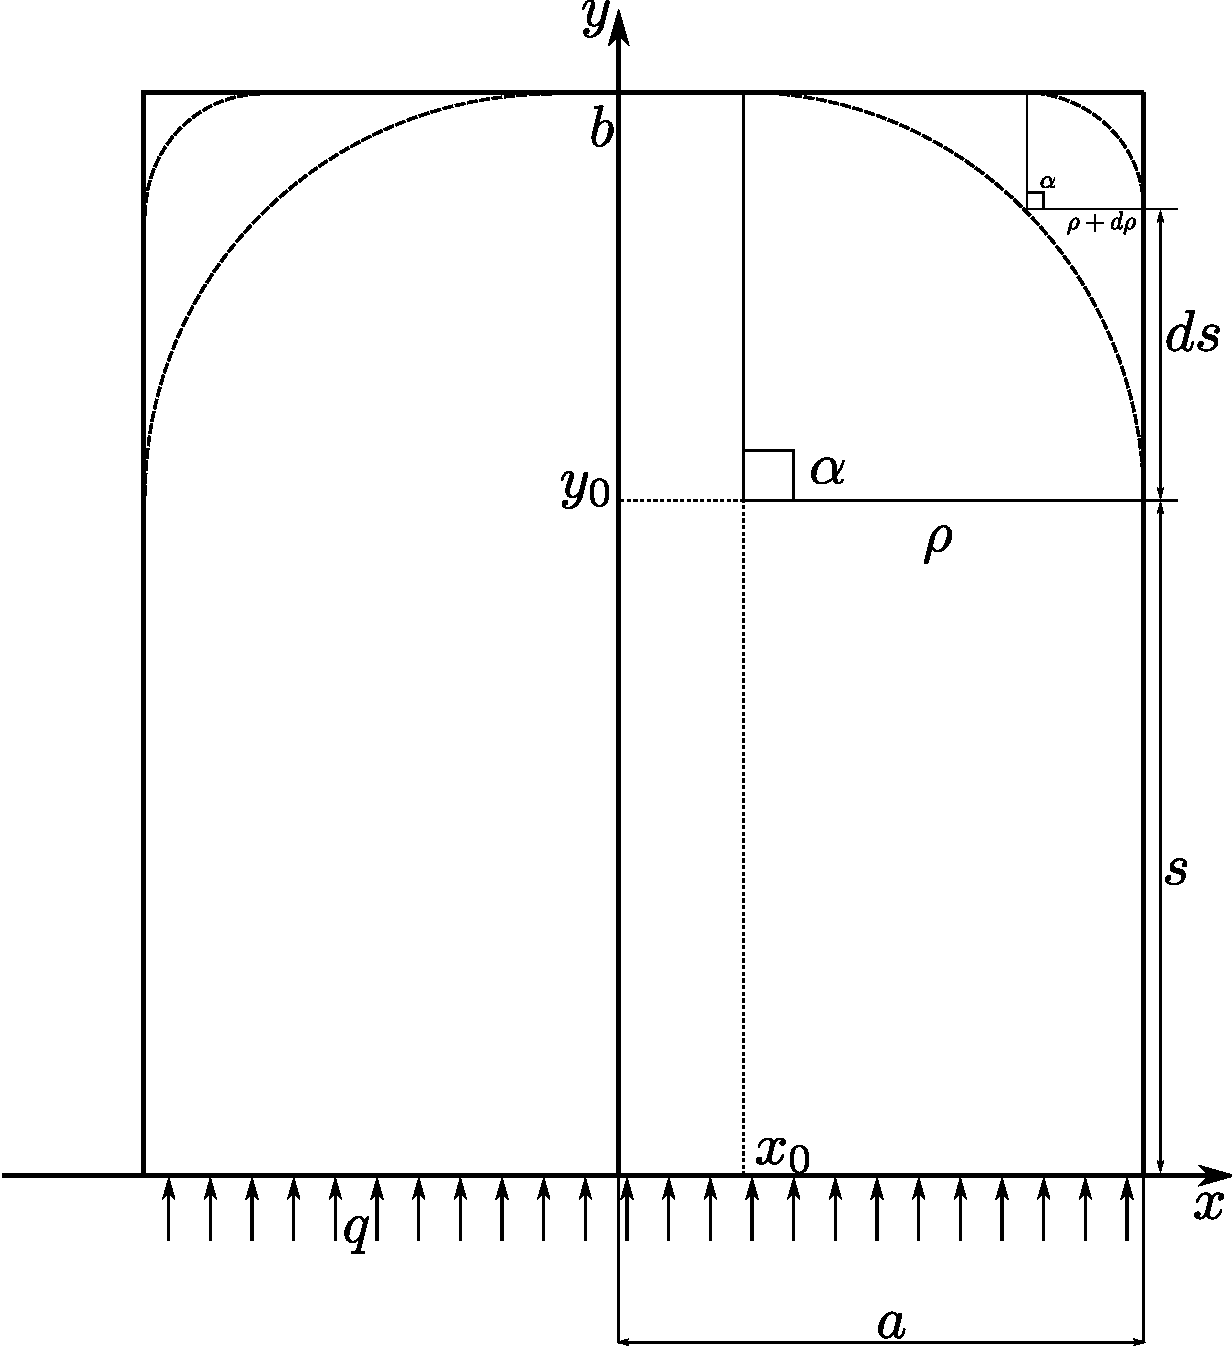
\includegraphics[width=1.0\linewidth]{images/vert_matrix2.pdf}}
                \caption{ Четвертая стадия }
				\label{vert_matrix_pic2}		
		\end{minipage}
		
	\end{figure}
	При рассмотрении матрицы с вертикальными стенками и плоским днищем учитывалось, 
	что стесненное деформирование проходит как две последовательные стадии: 
	третья стадия~--- когда мембрана касается только стенок матрицы и четвертая 
	стадия~--- когда мембрана касается днища матрицы и свободных дуг становится две.
	
	
	Дана матрица шириной $2a$ и высотой $L$.
	Рассмотрим два близких состояния в третьей стадии:
	одно  с радиусом $\rho$ и длиной участка контакта $s$ и с длиной участка контакта $s+ds$. При касании только вертикальных стенок радиус свободной дуги матрицы изменятся не будет, поэтому: 
\begin{equation}
dp = \dfrac{ds}{s+\frac{\pi}{2}\rho}
\label{vertikal_matrix_trird}
\end{equation}

Введем безразмерные величины:
\begin{equation}
\overline{\rho} = \dfrac{\rho}{\alpha}, \overline{s}=\dfrac{s}{a},
\label{parall_variables_no_dimention}
\end{equation}

Подставляя (\ref{parall_variables_no_dimention}) в (\ref{vertikal_matrix_trird}) и учитывая, что из геометрического смысла на этом этапе $\rho = a$, получим(черточки над безразмерными переменными опустим):
	\begin{equation}
	dp_\theta = \dfrac{ds}{s+\frac{\pi}{2}}
	\label{vertikal_matrix_trird_nodim}
	\end{equation}

Перейдем к координатам, аналогично пункту \ref{section_1_1} этой главы, введя тривиальную зависимость точки прилипания от крайней координаты касания: $s=y_0, ds = dy_0$.
Проведя замену переменных и учитывая условие несжимаемости плоского деформированного состояния получаем:
	\begin{equation}
	H=\dfrac{H_1(y+\frac{\pi}{2})}{\frac{\pi}{2}}
	\end{equation}
Поставляя (\ref{vertikal_matrix_trird_nodim}), (\ref{sigma}) в (\ref{main_equation}) и используя замену переменных получим:
\begin{equation}
t = t_1 + \int\limits_0^{y_0}\left[ \dfrac{2H}{\sqrt3 q \rho} -1\right]^n\left(\dfrac{dy_0}{y_0+\frac{\pi}{2}}\right)
\end{equation}
	где $t_1$~-- время окончания стадии свободного деформирования.   
Выражение подлежит численному исследованию, результаты которого приведены в главе \ref{chapter_2} пункте \ref{section22}.

	

	
	Рассмотрим два близких состояния при касании мембраны днища матрицы:
	одно  с радиусом $\rho$ и длиной участка контакта $s$ и другое с радиусом $\rho+d\rho$ с длиной участка контакта $s+ds$ (рис. \ref{vert_matrix_pic2}).
	
	Выражение окружной деформации примет вид:
	\begin{equation}
	% это формула для 4 стадии
	p_\theta = \dfrac{2ds+\frac{\pi}{2}d\rho}{b-a+2s+\frac{\pi}{2}},
	\label{vert4stadia}
	\end{equation}
   из рис. \ref{vert_matrix_pic2} видно, что $2a$ и $b$~--- ширина и глубина матрицы, $s$~--- как и в предыдущих обозначениях длина участка касания. Для удобства введем обозначения:
   \begin{equation}
   \overline{b} = \dfrac{b}{a}+\left(\dfrac \pi 2 -1\right),\; \overline{x} = \dfrac{s}{a}
	\label{vert_nodim_4}
   \end{equation}
	   
	
    Подставляя (\ref{vert_nodim_4}) в (\ref{vert4stadia}), дифференцируя по $t$ 
    и используя соотношение 
    \begin{equation} 
    p_u=\frac{2}{\sqrt 3}p_\theta
	\end{equation}
     получаем выражение(черточки над безразмерными величинами опущены):
    \begin{equation}
    \dot{p_u} = \dfrac{2}{\sqrt 3}\dfrac{\left( 2+\frac{\pi}{2}\right)}{b+\left(2-\frac{\pi}{2}x_0\right)},
    \label{vert_nodim}
    \end{equation}
	$x_0 \in [0, 1]$~-- так же как и в предыдущих обозначениях крайняя точка касания днища.
	
	Подставляя (\ref{vert_nodim}) в (\ref{main_equation}) получаем зависимость времени от точки касания:
	\begin{equation}
	t = t_2+ \int\limits_0^{y_0}\left[ \dfrac{2H}{\sqrt3 q \rho} -1\right]^n\left(\dfrac{\left( 2+\frac{\pi}{2}\right)dx_0}{b+\left(2-\frac{\pi}{2}x_0\right)}\right),
	\end{equation}
	
где $t_2$~-- время окончания третьей стадии деформирования, $H_2$~-- толщина мембраны, соответствующей $t_2$, а $H$ вычисляется по формуле:
\begin{equation}
 H = H_2/(1+(\dfrac{4}{\pi} - 1)x)
\end{equation}   

Выражение подлежит численному исследованию, результаты которого приведены в главе \ref{chapter_2} пункт \ref{section22}.

В случае постепенного прилипания контактная часть мембраны(с переменной толщиной)
является жесткой, недеформированной, а свободная часть мембраны(с постоянной толщиной), представляет собой часть дуги окружности.
разбивая процесс на две стадии, аналогично случаю скольжения получим соотношения для третьей стадии:

\begin{equation}
p_\theta = \dfrac{ds}{\frac{\pi}{2}\rho}
\label{stick_deformation_vert_matrix3}
\end{equation}

Проведя обозначения, аналогичные случаю скольжения получим: 
\begin{equation}
y_0 = \dfrac{s}{a}; \; \rho = a
\end{equation}

Тогда, аналогично выводам в случае идеального скольжения получим:
\begin{equation}
	dp_\theta = \dfrac{2dy_0}{\pi};
	\dot{p_u} = \dfrac{2}{\sqrt 3}\dfrac{2dy_0}{\pi},
\label{stick_deformation_vert_matrix3_final}
\end{equation}

Зависимость толщины мембраны от крайней точки касания на протяжении третьей стадии,
 в случае прилипания мембраны к стенке матрицы, будет иметь вид:
    
 \begin{equation}
   H = H_1 e^{-\frac{2}{\pi}y_0}
   \end{equation}
   
   Проведя подстановку (\ref{stick_deformation_vert_matrix3_final}) в (\ref{main_equation}):
 \begin{equation}
   t = t_1 + \int\limits^{y_0}_1 \left[ \dfrac{2H}{\sqrt3 q \rho} -1\right]^n\dfrac{2}{\pi}\,dy_0,
   \end{equation}

Проводя рассуждения, аналогичные четвертой стадии идеального скольжения и третьей стадии в условиях прилипания,  для четвертой стадии 
стесненного деформирования в условии прилипания получим основные соотношения:

 \begin{equation}
   p_\theta = \dfrac{(2ds+ \frac{\pi}{2}d\rho)}{\frac{\pi}{2}\rho}
 \end{equation}

Переходя к координатам и безразмерным величинам по формулам:

\begin{equation}
\overline{\rho} = \dfrac{\rho}{a} = 1-x_0, \; \overline{s} = \dfrac{s}{a}, d\overline{s} = dx_0, \; d\overline{\rho},
\end{equation}

где $x_0$~--- крайняя координата точки касания днища матрицы, получим соотношения, характеризующие деформированное состояние мембраны:

 \begin{equation}
   p\theta = \dfrac{(2-\frac{\pi}{2}) dx_0}{\frac{\pi}{2} (1-x_0)}
 \end{equation}
   
 \begin{equation}
   H = H_2 \dfrac{(\pi-x_0)^{4-\pi}}{\pi^{1-\pi}}
 \end{equation}
   
   Проведя подстановку (\ref{stick_deformation_vert_matrix3_final}) в (\ref{main_equation}):
 \begin{equation}
   t = t_2 + \int\limits^{y_0}_1 \left[ \dfrac{2H}{\sqrt3 q \rho} -1\right]^n\dfrac{(2-\frac{\pi}{2}) dx_0}{\frac{\pi}{2} (1-x_0)}\,dx_0,
   \end{equation}

Как при условии идеального скольжения так и при условии прилипания были проведены расчеты, результаты которых представлены в Главе 2.    

\section{Численное интегрирование}
В работе рассматриваются два метода приближенного вычисления интегралов
(\ref{simpson}, \ref{gauss}).

Все приемы численного интегрирования [\ref{samarskiy}] основаны на  замене определенного интеграла 
\begin{equation}
	I = \int\limits_a^b f(x)\,dx
\end{equation}
конечной суммой
\begin{equation}
	I_n = \sum\limits_{k=0}^n c_k f(x_k),
\end{equation}

где $c_k$~--- числовые коэффициенты и $x_k$~---точки отрезка $[a,b]$, $k=0, 1, \ldots, n$.
При этом интеграл по переменному верхнему пределу берется так: выбирается разбиение возможных значений верхнего предела
с определенным шагом. Внутри этого отрезка оба предела интеграла являются определенными и выбирается одна из ниже описанных формул.

\subsection{Метод Симпсона\label{simpson}}
При аппроксимации интеграла заменим подынтегральную функцию $f(x)$ параболой, проходящей через точки
($x_j, f(x_j) $), $j=i-1, i-0.5, i$. Подробный вывод формул представлен в [\ref{samarskiy}]. Приведем окончательную формулу:
\begin{equation}
\int\limits^b_a f(x)\,dx \approx \dfrac{b-a}{6N}\left[f_0 +f_{2N}+2(f_2+f_4+\ldots+f_{2N-2})+4(f_1+f_3+\ldots+f(2N-1))\right],
\end{equation}

где $2N$~--- количество узлов одномерной сетки c шагом $h$, $f_i$~--- значение функции $f$ в точке $x_i$. $x_i = a+kh$.

\subsection{Метод Гаусса\label{gauss}}
Повысить точность вычисления численного интеграла можно не только с помощью уменьшения шага интегрирования, но и за счет 
выбора определенных точек интегрирования. Уменьшение шага ведет в пропорциональному увеличению времени работы программы, что не
приемлемо по времени работы при сильно увеличивающейся точности.

Метод Гаусса описывает способ нахождения специальных точек интегрирования, при этом в разложении интеграла используются квадратурные
формулы наивысшей алгебраической точности.
Изначально при методе Гаусса рассматривается канонический интеграл:
\begin{equation}
\int\limits_{-1}^1 f(x)\, dx = \sum\limits_{i=1}^n w_i f(x_i)
\end{equation}

Для перехода к произвольному интервалу можно воспользоваться следующей заменой:
\begin{equation}
\int_a^b f(x)\,dx = \frac{b-a}{2} \int_{-1}^1 f\left(\frac{b-a}{2}z 
+ \frac{a+b}{2}\right)\,dz \approx \frac{b-a}{2} \sum_{i=1}^n w_i f\left(\frac{b-a}{2}z_i + \frac{a+b}{2}\right).
\end{equation}

В работах [\ref{samarskiy}, \ref{gauss_book}, \ref{gauss_article}] подробно описан вывод и доказательство корректности формул, поэтому просто приведем таблицу 
ключевых значений для 1,2,3,4,5-ти точечного метода.

\begin{center}

\renewcommand{\arraystretch}{2}
\begin{tabular}{|c|c|c|}
\hline
Кол-во точек    & $x_i$ & $w_i$ \\
\hline\hline
1    & 0  & 2\\[5pt] \hline
2     & $\pm\frac{\sqrt{3}}{3}$   & 1 \\[5pt] \hline
\multirow{2}{*}{3}    & 0  & $\frac 89$\\[5pt] \cline{2-3}
& $\pm \sqrt{\frac 3 5}$  & $\frac 5 9$\\[5pt] \hline

\multirow{2}{*}{4}    & $\pm\sqrt{\Big( 3 - 2\sqrt{\frac65} \Big)/7}$ & $\frac{18+\sqrt{30}}{36}$\\[5pt] \cline{2-3}
& $\pm\sqrt{\Big( 3 + 2\sqrt{\frac{6}{5}} \Big)/7}$ & $\frac{18-\sqrt{30}}{36}$\\[5pt] \hline

\multirow{3}{*}{5}    & 0 & $\frac{128}{225}$\\[5pt] \cline{2-3}
& $\pm\frac13\sqrt{5-2\sqrt{\frac{10}{7}}}$ & $\frac{322+13\sqrt{70}}{900}$\\[5pt] \cline{2-3}
& $\pm\frac13\sqrt{5+2\sqrt{\frac{10}{7}}}$ & $\frac{322-13\sqrt{70}}{900}$\\[5pt] \hline

\end{tabular}
\label{gauss_table}
\end{center}

В работе использовался пятиточечный метод и окончательная формула принимает вид:
\begin{equation}
\begin{split}
	\int\limits_a^b f(x)\,dx =  128/255 f(\dfrac{a+b}{2})+
  \dfrac{322+13\sqrt{70}}{900}\cdot f\left(\dfrac{a+b}{2} + \dfrac 13\cdot \sqrt{5-2\sqrt{\dfrac{10}{7}}}\cdot\dfrac{b-a}{2}\right) +\\
  \dfrac{322+13\sqrt{70}}{900}\cdot f\left(\dfrac{a+b}{2} - \dfrac 13\cdot \sqrt{5-2\sqrt{\dfrac{10}{7}}}\cdot\dfrac{b-a}{2}\right) +\\
  \dfrac{322-13\sqrt{70}}{900}\cdot f\left(\dfrac{a+b}{2} + \dfrac 13\cdot \sqrt{5+2\sqrt{\dfrac{10}{7}}}\cdot\dfrac{b-a}{2}\right) +\\
  \dfrac{322-13\sqrt{70}}{900}\cdot f\left(\dfrac{a+b}{2} - \dfrac 13\cdot \sqrt{5+2\sqrt{\dfrac{10}{7}}}\cdot\dfrac{b-a}{2}\right);
\end{split}
\end{equation}

\subsection{Погрешности}
Оценим погрешность, получаемую по двум рассмотренным методам интегрирования.
При вычислении интеграла 
\begin{equation}
\int\limits^b_af(x)\,dx
\end{equation}
методом Гаусса погрешность оценивается по формуле:  
\begin{equation}
R(n) = \dfrac{2^{2n+3}(n+1)!}{((2n+2)!)^3(2n+3)}f^{(2n+2)}(\xi),\; \xi \in [-1, 1]
\end{equation}

Вычисление производной 4 и 18 порядка в рассматриваемых подынтегральных функциях представляет определенные сложности,
поэтому оценка погрешности метода Гаусса производится по методу Ругге-Ромберга. При этом получается, что метод Гаусса 
обеспечивает восемнадцатый порядок точности. Широко распространена [\ref{samarskiy}] оценка метода Симпсона как $O(h^4)$.
Так как метод Симпсона брался с очень маленьким шагом на протяжении всего участка интегрирования, а метод Гаусса был пятиточечным, то вычисления по методу Симпсона оказались более точные, но следует отметить, что время работы метода Симпсона при уменьшении шага увеличивается не пропорционально быстро.